\subsubsection{Direct Memory Access (DMA)}
\label{sec:CubeMXDMA}

Die I\textsuperscript{2}S Schnittstellen unterstützen den automatischen Datentransfer über den DMA Controller. In der Abbildung \ref{pic:CubeMX_I2S_DMA} ist die Konfiguration für den Peripheral to Memory Kanal ersichtlich. Der Memory to Peripheral Kanal wird mit den selben Einstellungen konfiguriert. \texttt{Half Word} bedeutet eine Datenbreite von 16 Bit, was der bei der I\textsuperscript{2}S2 Schnittstelle (Abschnitt \ref{sec:CubeMXI2S}) eingestellten Datenwortbreite entspricht.

\begin{figure}[H]
	\centering
	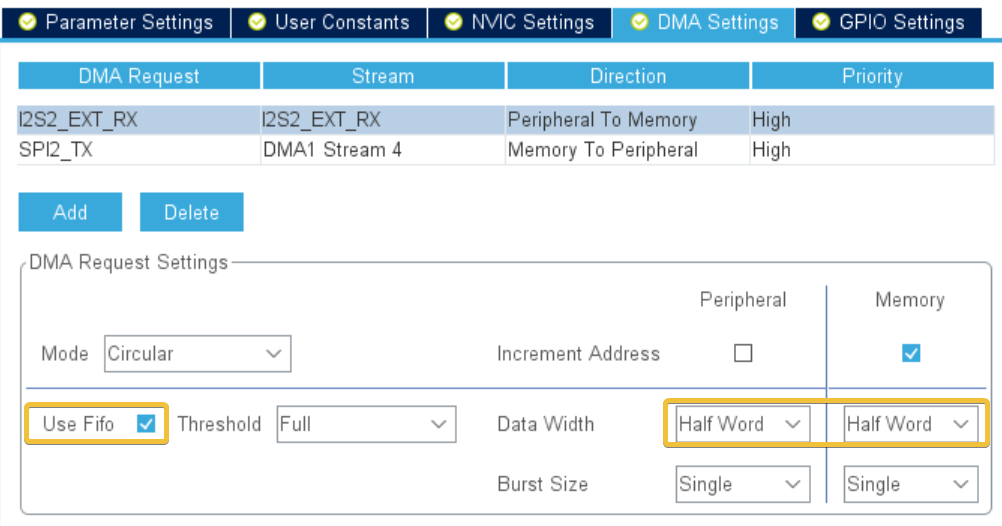
\includegraphics[width=0.9\linewidth]{CubeMX_I2S_DMA}
	\caption{DMA Einstellungen der I\textsuperscript{2}S2 Schnittstelle}
	\label{pic:CubeMX_I2S_DMA}
\end{figure}

